\documentclass{article}

\usepackage{tabu}
\usepackage{pbox}
\usepackage[margin=1in]{geometry}
\usepackage{xcolor}
\usepackage{amsmath}
\usepackage{graphicx}
\usepackage{setspace}

\frenchspacing
\setlength{\parskip}{1em}
\renewcommand{\arraystretch}{1.5}
\setlength\parindent{0pt}

\begin{document}

\section{MOSFETs}

\textbf{Definitions:}

\vspace{-5mm}
\begin{itemize} \itemsep0pt
	\item \(k_n \equiv \mu_nC_{ox} \frac{W}{L}\), \(k_p \equiv \mu_pC_{ox} \frac{W}{L}\)
	\item \(k'_n \equiv \mu_nC_{ox}\), \(k'_p \equiv \mu_pC_{ox}\)
	\item \(V_{OV} \equiv V_{GS}-V_{th}\)
	\item \(V_A \equiv \frac{1}{\lambda}\)
	\item \(V'_A \equiv \frac{V_A}{L}\)
	\item \(g_m \equiv \frac{\partial i_D}{\partial v_{GS}} = \frac{i_d}{v_{gs}}\)
\end{itemize}

\textbf{Large signal characteristics, \(k=k_n\) or \(k_p\) as appropriate:}

\begin{tabu}{  l  X  X  }
	\hline
	Region & Condition & Properties \\ \hline
	Saturation & \(|V_{GS}| > |V_{th}| \bigwedge |V_{DS}| \geq |V_{OV}|\) &
	\pbox{10cm}{
		\vspace{1mm}
		\(\begin{aligned}
					I_D &= \frac{k}{2} V_{OV}^2 (1+\frac{V_{DS}}{V_A}) \\
					&\approx \frac{k}{2} V_{OV}^2
		\end{aligned}\)
	}\\

	Triode & \(|V_{GS}| > |V_{th}| \bigwedge |V_{DS}| \leq |V_{OV}|\) &
	\pbox{10cm}{ \(I_D = k(|V_{OV}|-\frac{1}{2}|V_{DS}|)|V_{DS}|\) } \\

	Cutoff & \(|V_{GS}| \leq |V_{th}|\) & \(I_D = 0\)\\
	\hline
\end{tabu}

For N-channel devices, all absolute value operations can be ignored.

\vspace{5mm}
\textbf{Small signal characteristics (saturation only):}

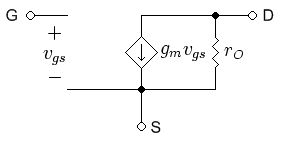
\includegraphics[height=100pt]{MOSFET_Small_Signal.png}\footnote{Image by Brews ohare at English Wikipedia} % https://commons.wikimedia.org/wiki/File:MOSFET_Small_Signal.png

\vspace{-5mm}
\begin{itemize}
	\item \(g_m = \frac{2I_D}{V_{OV}} = k|V_{OV}|\)
	\item \(r_o = \frac{V_A}{I_D}\)
\end{itemize}

\newpage
\section{BJTs}

\textbf{Definitions:}

\vspace{-5mm}
\begin{itemize} \itemsep0pt
	\item \(V_T \equiv \frac{kT}{q} \approx 25\text{mV}\)
	\item \(\alpha \equiv \frac{\beta}{\beta + 1}\)
	\item \(g_m \equiv \frac{\partial I_C}{\partial V_{BE}}\)
\end{itemize}

\textbf{Large signal characteristics:}

\begin{tabu}{  l  X  X  }
	\hline
	Region & Condition & Properties \\ \hline

	Saturation & Both junctions forward biased &
	\pbox{10cm}{
		\vspace{-5mm}
		\setstretch{1.2}
		\(|V_{BE}| \approx 0.7\text{V}\) \\
		\(|V_{CE}| \approx 0.2\text{V}\) \\
		\(|V_{BC}| \approx 0.5\text{V}\) \\
		\(I_C = \beta_{forced} I_B\)
	}
	\\[-13mm]

	Active & EB junction forward biased, CB junction reverse biased &
	\pbox{10cm}{
		\setstretch{1.3}
		\(\begin{aligned}
					I_C &= I_S e^{\frac{|V_{BE}|}{V_T}} (1 + \frac{V_{CE}}{V_A}) \\[-3mm]
						   &\approx I_S e^{\frac{|V_{BE}|}{V_T}}
		\end{aligned} \) \\
		\(I_C = \beta I_B\) \\
		\(I_E = \frac{I_C}{\alpha} = I_B + I_C\) \\
		\(|V_{BE}| \text{is effectively limited at around 0.7V}\)
	} \\[-5mm]

	Cutoff & Both junctions reverse biased & \(I_C = I_B = 0\) \\[1mm]
	\hline
\end{tabu}

For NPN devices, all absolute value operations can be ignored.

\vspace{5mm}
\textbf{Small signal characteristics (active only):}

TODO: image

\vspace{-5mm}
\begin{itemize}
	\item \(g_m = \frac{I_C}{V_T}\)
	\item \(r_{\pi} = \frac{\beta}{g_m} = \frac{V_T}{I_B}\)
	\item \(r_o = \frac{V_A}{I_C}\)
\end{itemize}

\end{document}
